\question \textbf{Backtrack with affine gap penalty}
  
Perform backtracking on E, F, and G tables to find the optimal alignment. The cells with double border should be visited during backtracking. 

\medskip 

\begin{figure}[h]
  \centering
      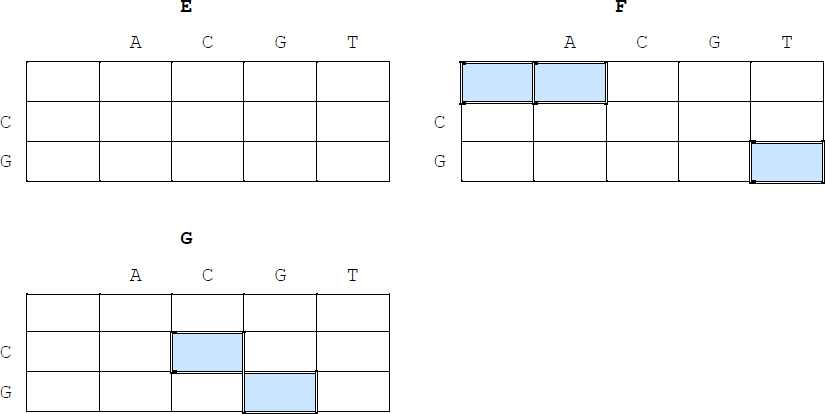
\includegraphics[width=0.75 \textwidth]{fig03/affine_dp_backtrack.png}
\end{figure}

\vspace{0.1 in}

\begin{parts}

%% (a)
  \part
   Write the optimal alignment.

  \begin{solution}[0.75 in]
  \begin{verbatim}
  q: -CG-
  d: ACGT
  \end{verbatim}
  \end{solution}

  \vspace{0.1 in}

\end{parts}

\newpage
